\documentclass[12pt, a4paper, titlepage]{report}
\usepackage[utf8]{inputenc}
\usepackage[IL2]{fontenc}
\usepackage[czech]{babel}
\usepackage[hidelinks]{hyperref}
\usepackage{svg}
\usepackage{graphicx}

\begin{document}

\begin{titlepage}
\begin{flushleft} 
{
\includegraphics{img/logo.png}\\[3cm]}
\end{flushleft}
\begin{center}

{\huge Rozpoznávání číslic neuronovou sítí\\[0.3cm]}
{\large KIV/PC – Semestrální práce\\[1.7cm]}
{\large Petr Kozler, A13B0359P\\}

\vfill
{\large \today}
\end{center}
\end{titlepage}

\tableofcontents

\newpage

\chapter{Zadání}
\par\noindent
Naprogramujte v~ANSI C přenositelnou \textbf{konzolovou aplikaci}, která jako vstup obdrží soubor obsahující snímek ručně psané číslice a soubor s~váhami a topologií již natrénované neuronové sítě s~dopředným šířením, na jejichž základě vytvoří v~paměti odpovídající neuronovou sít’ a následně provede klasifikaci obsahu zadaného snímku. Výstupem aplikace je třída snímku po klasifikaci, tzn. rozpoznaná číslice.
\par
Klasifikací se rozumí zařazení vstupních dat (v tomto případě snímku) do jedné z~\textit{N} tříd. V~úloze rozpoznávání ručně psaných číslic je pak \textit{N} = 10, protože klasifikujeme číslice 0, 1, 2, . . . , 9. V~případě, že se na snímku nachází ručně psaná číslice ”5“, odpovídající třída při správné klasifikaci je taktéž číslo 5.\\
\par\noindent
Program se bude spouštět příkazem:\\ \texttt{nnet.exe \textless soubor-se-sítí\textgreater \textless soubor-s-číslicí\textgreater}\\ a bude očekávat 2 parametry na příkazové řádce. Prvním parametrem bude jméno souboru s~daty neuronové sítě, která se použije pro klasifikaci. Druhým parametrem bude jméno souboru, který obsahuje obrazová data ručně psané číslice, kterou budete klasifikovat.\\
\par\noindent
Výsledný program tedy budete spouštět například tímto způsobem:
\par\noindent
\texttt{...\textbackslash\textless nnet.exe neuronova\_sit.txt vstupy\textbackslash0.dat}\\
\par\noindent
Nato program vypíše do konzole například znak: \texttt{2}
\par\noindent
čímž dá najevo, ze vstupní soubor \texttt{0.dat} ve složce \texttt{vstupy} obsahuje číslici ”2“.
\newpage\noindent
Pokud nebudou na příkazové řádce uvedeny oba dva argumenty, vypište chybové hlášení a stručný návod k~použití programu (v angličtině). Program v~tomto či jiném \textbf{chybovém stavu zároveň ukončete nenulovou návratovou hodnotou} (nulovou v~případě, ze vše proběhne v~pořádku).
\par
Ve složce texttt{vstupy} se nachází soubory obsahující vstupní soubory pro aplikaci. Pro náhled, jaké obrázky se skrývají uvnitř těchto binárních dat, můžete prozkoumat složku \texttt{nahledy}, ve které se zároveň nachází i textový soubor \texttt{\_tridy.txt} se správnými třídami pro každý vstupní soubor.\\
\par\noindent
Hotovou práci odevzdejte v~jediném archivu typu ZIP prostřednictvím automatického odevzdávacího a validačního systému. Archiv necht’ obsahuje všechny zdrojové soubory potřebné k~přeložení programu, \textbf{makefile} pro Windows i Linux (pro překlad v~Linuxu připravte soubor pojmenovaný \texttt{makefile} a pro Windows \texttt{makefile.win}) a dokumentaci ve formátu PDF vytvořenou v~typografickém systému \TeX, resp. \LaTeX. Bude-li některá z~částí chybět, kontrolní skript Vaší práci odmítne.\\
\par\noindent
\textsl{Úplné znění zadání semestrální práce s~upřesňujícími informacemi se nachází v~původním dokumentu zadání, který je ke stažení zde:\\}
\url{http://www.kiv.zcu.cz/studies/predmety/pc/doc/work/sw2014-02.pdf}

\newpage

\chapter{Analýza úlohy}
Zadaná úloha přináší následující hlavní dílčí problémy: validace vstupních parametrů, čtení dat ze vstupních souborů, způsob uložení těchto dat do paměti a výpočet aktivace neuronů pro klasifikaci vstupního snímku.
\section{Validace vstupních parametrů}
Při ověřování korektního zadání vstupních parametrů je vhodné nejprve ověřit, zda byly zadány ve správném počtu. Zjevně správný počet parametrů je právě 3, neboť první parametr v~jazyce C představuje vždy cestu ke spuštěnému programu, zbylé dva parametry pak cesty k~souborům se vstupními daty, kdy první z~nich obsahuje informace o natrénované neuronové síti a druhý snímek číslice. \par
Po ověření počtu vstupních parametrů se tedy program přesvědčí, zda poslední dva parametry obsahují cesty k~platným existujícím souborům. Pokud ano, zahájí načítání vstupních dat.
\section{Čtení vstupních dat}
Program načte nejprve snímek s~číslicí, který bude představovat vstupní vrstvu neuronové sítě (podrobněji popsáno níže) a poté soubor se sítí, na základě kterého jsou vytvořeny ostatní vrstvy prozatím bez vypočtených aktivací jednotlivých neuronů. Formát jednotlivých souborů je značně odlišný, proto i jejich čtení je řešeno různými způsoby.
\subsection{Čtení snímku číslice}
Soubor představující snímek ručně psané číslice je binární a neobsahuje žádnou hlavičku, pouze samotná data. Daty se zde myslí jednotlivé body snímku. Ze specifikace souboru snímku v~původním dokumentu zadání vyplývá, že body jsou reprezentovány 32-bitovými (4 byty) číselnými hodnotami typu \texttt{float} (desetinné číslo s~plovoucí řádovou čárkou) ve formátu \texttt{IEEE 754} (obr.~\ref{fig:ieee}) a bitovém pořadí \texttt{Little Endian} (obr.~\ref{fig:le}). Hodnota představuje intenzitu barvy v~daném bodě snímku, pro jednoduchost jsou tedy předpokládány pouze snímky ve stupních šedi (obr.~\ref{fig:digit}). \par
Data jsou čtena po jednotlivých čtveřicích bytů pomocí funkce \texttt{fread()}, přičemž nejméně významný byte je uložen do paměti i přečten z~paměti jako první. Převod uložené čtveřice bytů na číslo typu \texttt{float} by bylo samozřejmě možné realizovat "ručně", určením znaménka z~prvního bitu, výpočtem exponentu z~dalších 8 bitů a mantisy z~posledních 23 bitů a z~těchto hodnot určit číslo, takový způsob je však v~ANSI C zbytečně složitý. Podstatně jednodušší je využití konstrukce \texttt{union}, se kterou můžeme data uložit jako pole 4 bytů (datový typ \texttt{char}) a poté k~nim jednoduše přistupovat rovnou jako k~číselné hodnotě (podrobněji v~popisu implementace níže).
\begin{figure}[htbp]
    \centering
    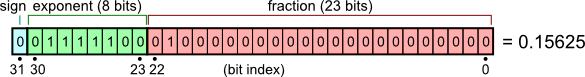
\includegraphics[width=12cm]{img/ieee.png}
    \caption{znázornění float hodnoty uložené v paměti be formátu IEEE 754}
    \label{fig:ieee}
\end{figure}
\begin{figure}[htbp]
    \centering
    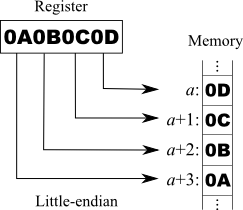
\includegraphics[width=6cm]{img/le.png}
    \caption{znázornění způsobu uložení bytů v pořadí Little Endian}
    \label{fig:le}
\end{figure}
\begin{figure}[htbp]
    \centering
    
\includegraphics[width=3cm]{img/digit.png}
    \caption{příklad snímku s číslicí}
    \label{fig:digit}
\end{figure}
\subsection{Čtení neuronové sítě}
Soubor, který představuje natrénovanou neuronovou síť (obr.~\ref{fig:nnet}), má textovou podobu, přičemž jako znak konce řádku je zde použita sekvence \texttt{\textbackslash CR\textbackslash LF}. První řádek souboru obsahuje číselný údaj o počtu vrstev neuronové sítě (nezahrnuje vstupní vrstvu).\par
Řádek je ve tvaru \texttt{Pocet vrstev:} \textit{n}, kde \textit{n} představuje číslo, které je třeba v~programu uložit jako celočíselnou hodnotu. Jako jednoduchý způsob bylo zvoleno načtení řádku pomocí funkce \texttt{fgets()}, následné rozdělení řetězce na tokeny podle znaku ":" a převod druhého tokenu, který tak již obsahuje pouze číslice popř. bílé znaky, na hodnotu typu \texttt{int} pomocí funkce \texttt{atoi()}. Další možností by mohlo být použití funkce \texttt{scanf()}. Pro přehlednost byla nicméně používána funkce \texttt{fgets()} v~průběhu celého čtení souboru.\par
Po řádku udávajícím počet vrstev již následují popisy jednotlivých vrstev vždy v~pořadí "popis hran – popis neuronů". Každý popis začíná vždy řádkem ve tvaru \texttt{W hodnoty vrstvy} \textit{k}\texttt{:} pro popis hran, resp. \texttt{b hodnoty vrstvy} \textit{k}\texttt{:} pro popis neuronů, kde \textit{k} značí index aktuální vrstvy.\par
Zde je nad načteným řetězcem opět použita sekvence volání funkce \texttt{strtok()}, ale tentokrát je řetězec rozdělen nejprve podle mezer, načež poslední token je teprve rozdělen podle znaku ":" a na celé číslo je pak funkcí \texttt{atoi()} převeden první token z~tohoto podřetězce.\par
Po řádcích, které udávají index vrstvy, již následují řádky obsahující pouze mezerou oddělené číselné hodnoty pro jednotlivé hrany, resp. neurony. Při popisu hrany má řádek tvar \textit{i} \textit{j} \textit{w}, kde \textit{i} a \textit{j} jsou celá čísla představující indexy neuronů, které hrana propojuje (\textit{i} je index neuronu v~předchozí vrstvě a \textit{j} ve vrstvě aktuálně popisované) a \textit{w} je reálné číslo představující váhu hrany. Při popisu neuronu má řádek tvar \textit{i} \textit{b}, kde \textit{i} je index neuronu v~aktuálně popisované vrstvě a \textit{b} je nezávislá konstanta, která se během výpočtu aktivace popisovaného neuronu přičte k~sumě vstupních aktivací.
Pro oddělení jednotlivých číselných hodnot na řádku je opět použita funcke \texttt{strtok()}, oddělovacím znakem je mezera, pro převod celočíselných hodnot z~pole znaků na typ \texttt{int} je použita opět funkce \texttt{atoi()} a pro převod desetinných hodnot na typ \texttt{float} je obdobně využito funkce \texttt{atof()}.
\begin{figure}[htbp]
    \centering
    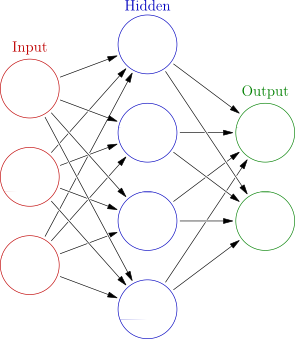
\includegraphics[width=6cm]{img/nnet.png}
    \caption{příklad neuronové sítě (znázornění neuronů a hran)}
    \label{fig:nnet}
\end{figure}
\section{Uložení dat v~paměti}
Neuronová síť je tvořena dvěma typy „objektů“ - neurony a hranami. Oba jsou ve finální podobě programu uloženy v~paměti podobným způsobem, nicméně při analýze byly zváženy i způsoby výrazněji odlišné.
\subsection{Uložení neuronů}
Pro uložení neuronů se nabízejí dva možné způsoby jak z~hlediska uložení jednotlivých prvků, tak z~hlediska jejich svázání do vrstev. Jednotlivé neurony je možné reprezentovat buď jedinou proměnnou typu \texttt{float}, která před výpočtem aktivací bude představovat konstantu \textit{b} a po výpočtu samotnou aktivaci, nebo jednotlivé hodnoty uložit odděleně a pro jednotlivé neurony svázat použitím konstrukce \texttt{struct} (struktura).\par
Pro vytvoření vrstev neuronů byly rovněž zváženy dva různé způsoby. První způsob je více "statický" – spočívá v~přečtení vstupního souboru sítě dvěma průchody, kdy prvním průchodem se spočítáním příslušných řádků určí počet neuronů v~dané vrstvě (neplatí pro vstupní vrstvu představovanou souborem se snímkem – tam postačí odvodit počet neuronů z~velikosti souboru a velikosti typu float ve formátu \texttt{IEEE 754}, konkrétně vydělit první jmenovanou hodnotu hodnotou druhou), následně se najednou alokuje veškerá potřebná paměť pro pole neuronů a při druhém průchodu příslušnou částí souboru se hodnoty teprve uloží do pole. Prvky takového pole mohou být ukazatele na strukturu představující neuron, ale nejjednodušší možností je kombinace tohoto způsobu s~reprezentací neuronu jako jediného čísla typu \texttt{float}, přičemž jeho pozice ve vrstvě je dána indexem v~poli \texttt{float} čísel. Druhý způsob vytvoření vrstvy již vyžaduje reprezentaci neuronu strukturou, kdy jednou z~položek struktury je ukazatel na další neuron, čímž je utvořen spojový seznam (obr.~\ref{fig:list}) neuronů.\par
Pro přehlednost a jednodušší načítání vstupních dat byl použit stejný způsob pro neurony i hrany. Pro obojí byla definována struktura a vrstvy byly vytvářeny jako spojové seznamy. Výhodou reprezentace vrstev neuronů jako pole čísel typu \texttt{float} by byla pravděpodobně vyšší rychlost programu a takové řešení by patrně bylo vhodnější při práci s~většími daty, nicméně pro testovací data se i rychlost použitého řešení ukázala jako uspokojivá.
\begin{figure}[htbp]
    \centering
    
\includegraphics[width=12cm]{img/list.png}
    \caption{příklad spojového seznamu (jedna z položek obsahuje hodnotu, druhá ukazatel)}
    \label{fig:list}
\end{figure}
\subsection{Uložení hran}
Pro reprezentaci hrany je již velmi vhodné použití struktury a s~ním i vytváření spojového seznamu, neboť každá hrana má dva indexy, které představují indexy neuronů, které propojuje. Dále musí uchovávat hodnotu představující váhu.
\section{Výpočet aktivací}
Posledním krokem nezbytným pro klasifikaci vstupního snímku pomocí neuronové sítě s~dopředným šířením je výpočet hodnoty aktivace každého jednotlivého neuronu.
Výpočet aktivace neuronu s~indexem \textit{j} ve vrstvě s~indexem \textit{k} je proveden s~užitím následujícího vzorce:
\par\noindent
$$x_{k,j} = tanh\left(b_{k,j} + \sum\limits_{i=1}^n x_{k-1,i} \cdot w_{k-1,j,i}\right)$$
\par\noindent
Hodnota $b_{k,j}$   je konstanta přiřazená danému neuronu ze vstupních dat a netřeba ji počítat. Druhým sčítancem ve funkci \texttt{tanh()} ve vzorci je suma součinů hodnot aktivace neuronů a váhy hran v~předchozí vrstvě s~indexem \textit{k} – 1. Zřejmě je zde tedy nutné použít cyklus, kde řídící proměnná i představuje index aktuálního neuronu v~součtu, jehož hodnota aktivace je vynásobena vahou hrany, pro kterou je splněna podmínka, že propojuje neuron z~vrstvy \textit{k} – 1 s~indexem \textit{i} (aktuální prvek v~součtu) a neuron z~vrstvy \textit{k} s~indexem \textit{j} (neuron, pro který je aktuálně prováděn výpočet). \par
Při hledání hrany splňující tuto podmínku je nutné neustále procházet spojový seznam. Taková operace má časovou složitost O(\textit{n}) a je tedy vhodné provést optimalizaci. Při výpočtu aktivace neuronu \textit{j} ve vrstvě \textit{k} zřejmě není nutné procházet celý spojový seznam hran vystupujících z~vrstvy \textit{k} – 1, ale pouze takové hrany, které ve vrstvě \textit{k} vstupují do neuronu \textit{j}. Před výpočtem sumy vstupních aktivací je tedy vytvořen dočasný spojový seznam, obsahující pouze takové hrany. Při výpočtu sumy je pak testován podstatně menší počet hran a stačí ověřovat pouze podmínku, že daná hrana ve vrstvě \textit{k} – 1 vystupuje z~neuronu \textit{i}.
Výpočet začíná u prvního neuronu ve vrstvě, která je nejblíže vrstvě vstupní (hodnoty aktivace neuronů ve vstupní vrstvě představují vstupní hodnoty z~jednotlivých bodů snímku). Po výpočtu všech neuronů v~dané vrstvě se analogicky pokračuje neurony v~další vrstvě směrem k~vrstvě výstupní.\par
Funkce \texttt{tanh()} pro výpočet hyperbolického tangentu je součástí standardní knihovny funkcí deklarovaných hlavičkovým souborem \texttt{math.h} a není tudíž nutné používat druhý vzorec uvedený v~původním dokumentu zadání.

\newpage

\chapter{Popis implementace}
Zdrojový kód programu je rozdělen do 10 samostatných souborů, z~toho 5 modulů a 5 hlavičkových souborů, jejichž podrobnější popis následuje níže.
\section{Hlavičkové soubory}
Hlavičkové soubory obsahují pouze definice uživatelských typů, preprocesorem vložených konstant a prototypy funkcí.
\subsection{Hlavičkový soubor defs.h}
Obsahuje pouze makra preprocesoru definující konstanty, které mohou být použity v~různých částech programu. 
\subsection{Hlavičkový soubor neuron.h}
Obsahuje prototypy funkcí pro práci se spojovým seznamem neuronů a definuje samotnou strukturu neuronu jako typ \texttt{neuron\_t}. Struktura neuronu obsahuje 4 položky. Jednak obsahuje celočíselnou hodnotu představující index neuronu a dvě \texttt{float} hodnoty – jedna představuje počáteční konstantu \textit{b}, druhá hodnotu aktivace. První dvě hodnoty jsou inicializovány při čtení vstupních dat a v~průběhu zpracování se jejich hodnoty již nemění. Třetí hodnota je určena po výpočtu aktivace daného neuronu. Poslední položkou struktury je ukazatel na další prvek spojového seznamu. Struktura neuronu je použita v~modulech \texttt{load.c} i \texttt{classify.c}.
\subsection{Hlavičkový soubor edge.h}
Obdoba souboru neuron.h pro hranu definovanou jako typ \texttt{edge\_t}. Struktura hrany obsahuje rovněž 4 položky – dvě celočíselné, které udávají indexy neuronů propojených danou hranou a jednu typu float, udávající váhu hrany. Analogicky ke struktuře neuronu i zde je poslední proměnnou opět ukazatel na další prvek ve spojovém seznamu. Struktura hrany je použita ve stejných modulech, jako struktura neuronu.
\subsection{Hlavičkový soubor load.h}
Soubor obsahující prototypy funkcí pro práci se vstupními soubory, resp. načtení vstupních dat a vytvoření odpovídajících datových struktur v~paměti. Kromě toho definuje pomocný typ \texttt{pixel\_t} jako svaz o 2 položkách. První položkou je pole bytů o velikosti shodné s~velikostí datového typu \texttt{float} v~bytech (4). Druhou položkou je reálné číslo typu \texttt{float}. Při načítání obrazových bodů vstupního snímku ze souboru je zde využito toho, že svaz uchovává vždy pouze jednu z~položek a k~uloženým datům tak lze přistupovat jako k~hodnotám různých datových typů. Konkrétní využití zde spočívá v~tom, že čtveřice bytů je zde uložena do pole a následně použita jako hodnota typu \texttt{float} při vytváření vstupní vrstvy neuronové sítě.
\subsection{Hlavičkový soubor classify.h}
Soubor obsahující prototypy funkcí pro výpočty nad vstupními daty a jejich klasifikaci.
\section{Moduly}
Moduly obsahují samotný výkonný kód programu.
\subsection{Modul main.c}
Řídící modul, obsahuje vstupní funkci programu, funkci pro výpis návodu k~použití programu do konzole, pro validaci vstupních parametrů příkazové řádky a pro volání funkcí pro načtení vstupních dat v~modulu \texttt{load.c} a jejich zpracování v~modulu \texttt{classify.c} a výpis výsledku zpracování (klasifikace snímku) do konzole.
\subsection{Modul neuron.c}
Obsahuje funkci pro vytvoření spojového seznamu neuronů (alokaci paměti pro první prvek, pokud předaný ukazatel na první prvek v~seznamu neuronů ukazuje na \texttt{NULL}), popř. vytvoření (alokaci paměti a inicializaci položek struktury předanými hodnotami) a vložení dalšího prvku na začátek předaného spojového seznamu (pokud ukazatel ukazuje na existující spojový seznam). Dále obsahuje funkci pro odstranění všech prvků předaného spojového seznamu a uvolnění alokované paměti.
\subsection{Modul edge.c}
Obsahuje funkce analogické k~funkcím v~modulu \texttt{neuron.c}, ale tentokrát pro strukturu hrany. Funkce z~obou modulů jsou použity ve funkcích definovaných v~modulech \texttt{load.c} a \texttt{classify.c}.
\subsection{Modul load.c}
Slouží k~načítání vstupních dat a sestavení odpovídajících datových struktur. Nejprve je v~hlavním modulu programu volána funkce, která přečte soubor se snímkem číslice a vytvoří spojový seznam neuronů představující vstupní vrstvu sítě. Následuje volání funkce, která řídí čtení souboru se sítí. Nejprve přečte první řádek souboru, ze kterého zjistí počet vrstev a podle toho alokuje potřebnou paměť pro pole ukazatelů na spojové seznamy neuronů a hran představující jednotlivé vrstvy. Obě pole jsou posléze předána funkci, která řídí čtení popisů jednotlivých vrstev. Tato funkce podle zjištěného počtu vrstev provede odpovídající počet volání funkcí pro čtení hodnot pro jednotlivé hrany a neurony (obě funkce jsou podobné a využívají pomocnou funkci pro získání indexu aktuálně popisované vrstvy z~řádku uvozujícího seznam hran, resp. neuronů v~dané vrstvě) a vytvoření spojových seznamů tvořících další vrstvy sítě, které uloží do předem alokovaných polí. Tím je vytvoření neuronové sítě v~paměti dokončeno. Nakonec je síť předána funkci pro zpracování v~modulu \texttt{classify.c}, jejíž návratová hodnota je předána do funkce v~hlavním modulu programu pro výpis výsledku.
\subsection{Modul classify.c}
Slouží ke zpracování načtených vstupních dat. První funkcí modulu, která je při běhu programu volána, je funkce, která nejprve postupně pro každý neuron každé vrstvy zavolá funkci pro výpočet aktivace daného neuronu. Tato funkce nejprve předá řízení funkci pro vytvoření dočasného seznamu hran (obsahuje pouze hrany potřebné pro výpočet aktivace aktuálního neuronu, což podstatně snižuje čas potřebný k~procházení spojového seznamu hran). v~takto vytvořeném seznamu pak pro každý neuron z~předcházející vrstvy zavolá funkci pro nalezení hrany, která jej propojuje s~aktuálně vyhodnocovaným neuronem (pokud existuje). Po dokončení výpočtu pro daný neuron provede uvolnění paměti alokované pro dočasný spojový seznam. Po dokončení výpočtu aktivací všech neuronů je volána funkce, která projde seznam neuronů ve vstupní vrstvě a vrátí index neuronu s~nejvyšší hodnotou aktivace, který představuje třídu, kam jsou zařazena vstupní data. Před předáním návratové hodnoty ještě dochází k~volání funkce pro systematické uvolnění paměti. Nejprve jsou smazány jednotlivé spojové seznamy neuronů a hran v~polích ukazatelů. Nakonec je uvolněna i paměť alokovaná pro jednotlivá pole.

\newpage

\chapter{Uživatelská příručka}
Pro automatický překlad a sestavení programu ze zdrojových souborů pomocí souboru \texttt{makefile} je vyžadován překladač \textbf{Microsoft Visual C/C++} nebo \textbf{GCC} (GNU Compiler Collection) a nástroj \textbf{Make}. Případně je teoreticky možné pro ruční překlad a sestavení zdrojových souborů programu použít jiný nástroj, například \textbf{Open Watcom C/C++}.\\
\par\noindent
Postup pro překlad a sestavení programu se mírně liší v~závislosti na operačním systému:
\section{Sestavení programu na systému Windows}
\begin{enumerate}
\item Otevřít \textbf{příkazovou řádku},
\item Použít příkaz \texttt{cd} pro přesun do adresáře se zdrojovými soubory a souborem \texttt{makefile.win},
\item Spustit překlad a sestavení programu příkazem \texttt{nmake -f makefile.win} (obr.~\ref{fig:cmd}) - je možné, že bude předtím nutné spustit dávkový soubor \texttt{vcvars32.bat} pro nastavení prostředí.
\end{enumerate}
\begin{figure}[htbp]
    \centering
    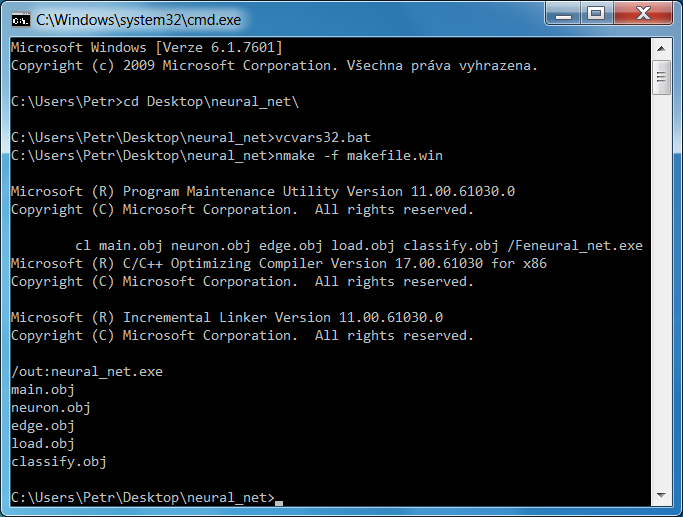
\includegraphics[width=12cm]{img/cmd.png}
    \caption{ukázka sestavení programu v příkazové řádce Windows}
    \label{fig:cmd}
\end{figure}
\section{Sestavení programu na systému Linux}
\begin{enumerate}
\item Otevřít \textbf{terminál},
\item Použít příkaz \texttt{cd} pro přesun do adresáře se zdrojovými soubory a souborem \texttt{makefile},
\item Spustit překlad a sestavení programu příkazem \texttt{make} (obr.~\ref{fig:term}).
\end{enumerate}
\begin{figure}[htbp]
    \centering
    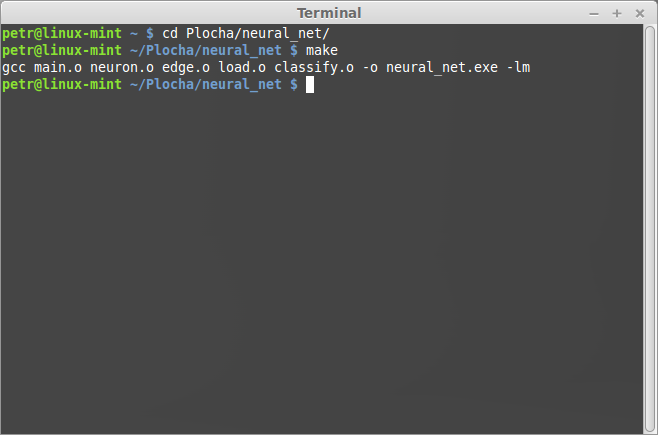
\includegraphics[width=12cm]{img/term.png}
    \caption{ukázka sestavení programu v terminálu Unix/Linux}
    \label{fig:term}
\end{figure}
\section{Spuštění programu}
Po sestavení by v~adresáři se zdrojovými soubory (obr.~\ref{fig:dir}) měl být vytvořen spustitelný soubor programu s~názvem \texttt{neural\_net.exe}, který lze spustit z~terminálu / příkazové řádky s~předáním vstupních parametrů představujících cesty ke vstupním souborům s~neuronovou sítí a se snímkem číslice. Příkaz pro spuštění programu z~terminálu / příkazové řádky je ve tvaru:
\par\noindent
\texttt{neural\_net.exe \textless soubor-se-sítí\textgreater \textless soubor-s-číslicí\textgreater}
\par\noindent
Specifikace vstupních souborů je uvedena v~kapitole \textbf{Analýza úlohy}. Po dokončení zpracování souborů program vypíše číselnou hodnotu odpovídající ručně psané číslici ze vstupního snímku (obr.~\ref{fig:run}).
\begin{figure}[htbp]
    \centering
    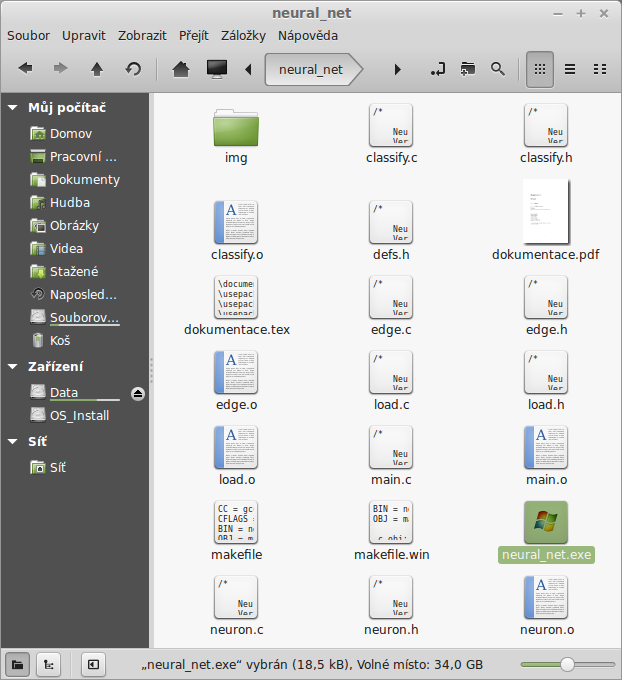
\includegraphics[width=12cm]{img/dir.png}
    \caption{ukázka adresáře s vytvořeným spustitelným souborem}
    \label{fig:dir}
\end{figure}
\begin{figure}[htbp]
    \centering
    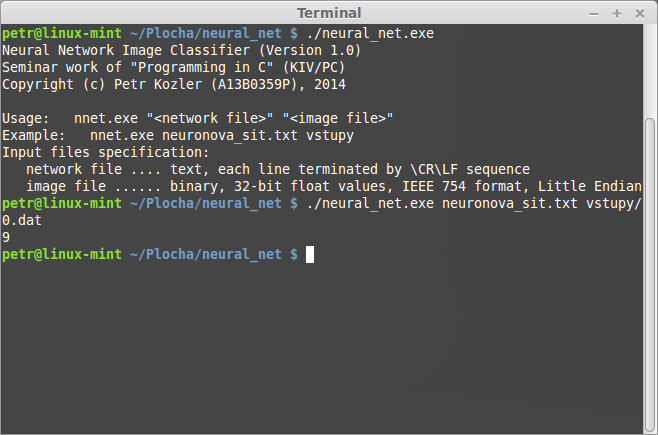
\includegraphics[width=12cm]{img/run.png}
    \caption{ukázka výstupu programu při spuštění bez parametrů a se správnými parametry}
    \label{fig:run}
\end{figure}

\newpage

\chapter{Závěr}
Program pro každý ze 30 testovacích snímků provedl správnou klasifikaci a před svým ukončením korektně uvolnil alokovanou paměť. Algoritmus vytvoření neuronové sítě a výpočtu aktivací neuronů byl navržen tak, aby fungoval obecně, tedy pro libovolný počet neuronů a libovolný počet vrstev. v~případě vložení nesprávných vstupních parametrů program reaguje výpisem chybového hlášení a stručného návodu k~použití programu. Aplikace má konzolovou podobu a je možné ji přeložit a spustit jak na systému Win32/64, tak na systému typu Unix/Linux. Lze tedy konstatovat, že zadání úlohy bylo v~základu splněno.\par
Čas běhu programu pro 1 snímek se pohyboval okolo 3s, což je hodnoceno jako uspokojivé (průměrný čas běhu obdobného programu psaného v~jazyce Java byl zhruba čtyřnásobný, což lze pravděpodobně přičíst časové režii spojené s~automatickou správou paměti), nicméně jak již bylo uvedeno v~analýze úlohy, pro práci s~většími daty by patrně bylo vhodné zvolit jiný přístup pro ukládání a práci s~neurony (ukládat vrstvy neuronů pouze jako pole hodnot typu \texttt{float}, jejichž velikost by byla buď zjišťována ze vstupních souborů, nebo v~méně obecném případě zvolena “staticky” jako shodná se vstupní vrstvou a přebytečná paměť poté uvolněna).\par
Dalším možným a žádoucím vylepšením by byla implementace podrobné kontroly korektního formátu vstupních dat, kdy při zjištění chyby by program reagoval buď okamžitým ukončením s~nenulovým návratovým kódem, nebo by např. vhodné chybějící hodnoty odhadl a pokusil se provést zpracování s~chybou, přičemž by vypsal hlášení o nalezené chybě.\par
Nad rámec zadání se jako další možné rozšíření nabízí vytvoření grafického uživatelského rozhraní pro pohodlnější ovládání programu.
\end{document}
